\appendix
\addappheadtotoc
%\addcontentsline{toc}{chapter}{Appendices}
\chapter{Yelp Dataset}\label{app:dataset}

Yelp is a US-based company whose goal is: ``to connect people with great local businesses.''\footnote{\url{https://yelp.com/about}}
It provides both mobile and web interface listing businesses such as restaurants or shopping centres.
Users can easily post a review for any business based on their recent visit.
Its convenience and usefulness makes the platform very popular.

It works in a similar manner like other recommnedation systems such as IMDB\footnote{Internet Movie Database \url{https://www.imdb.com/}} or
TripAdvisor.\footnote{\url{https://www.tripadvisor.com}}
There are restaurant profiles to which users can add reviews.
Users can search for restaurants based on various parameters as shown in \autoref{fig:filters}.

\begin{figure}[ht]\centering
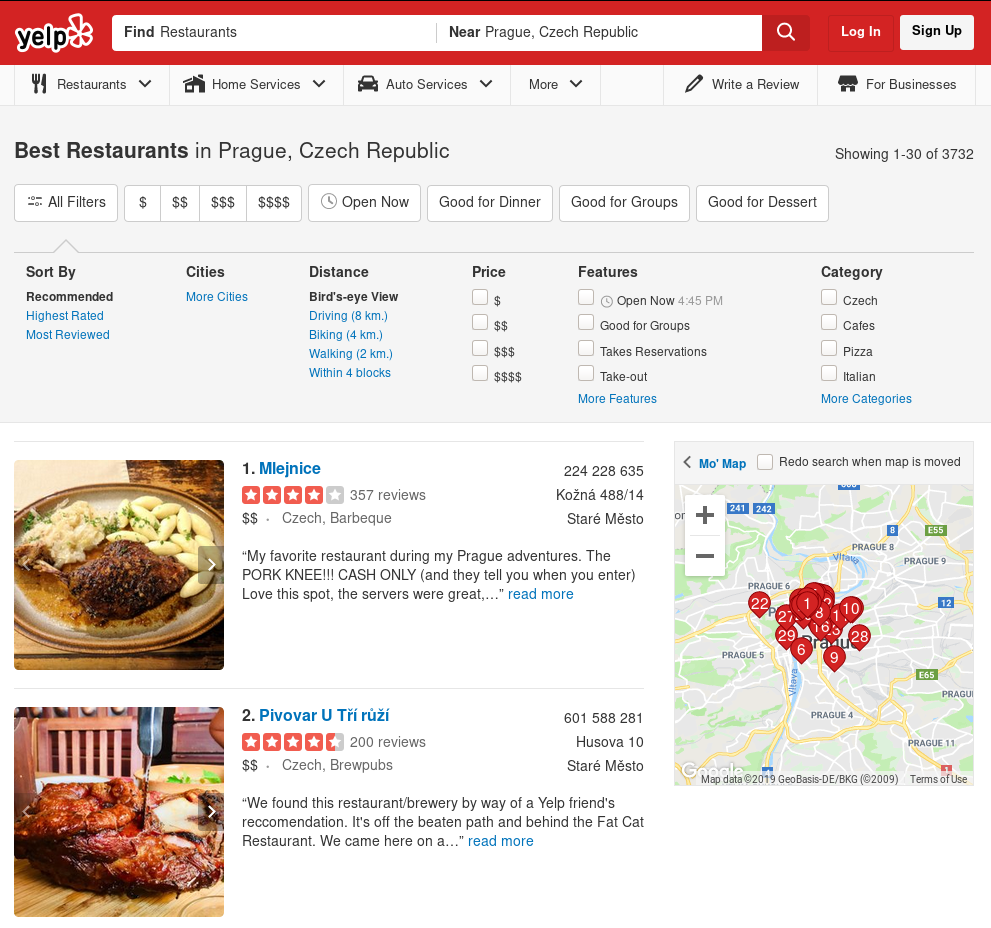
\includegraphics[width=130mm]{../img/filters.png}
\caption{Seeking restaurants with parameters}
\label{fig:filters}
\end{figure}

An example of a profile is shown in \autoref{fig:dobra_trafika}.
On the sides, various information such as price range or opening time is shown.
The main part is devoted to reviews.
Every review clearly displays the number of stars awarded and the text.
Also, Yelp already works with some sort of usefulness,
because two reviews have been hidden as can be seen in the bottom of the picture.

Yelp also allows users to flag properties of other reviews in the form of \emph{likes}.
Each review has three buttons --- \emph{useful}, \emph{funny} and \emph{cool} as can be seen in \autoref{fig:dobra_trafika}.
A user can vote for the property of a review by clicking on one of these buttons.

\begin{figure}[ht]\centering
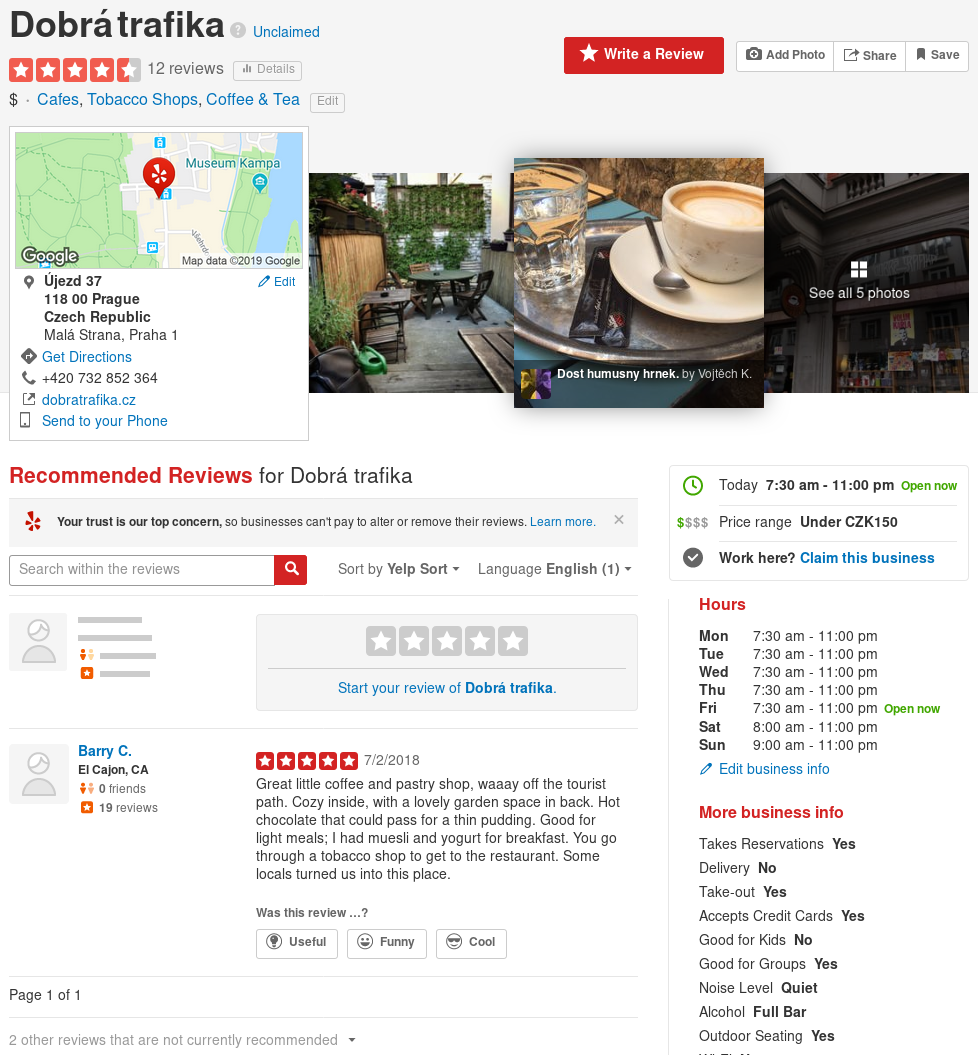
\includegraphics[width=130mm]{../img/dobra_trafika.png}
\caption{An example of an online profile}
\label{fig:dobra_trafika}
\end{figure}

There are three main reasons we chose Yelp reviews.

First, this platform is very popular and as such has sufficient data.

Secondly, the company publishes every year an open dataset which can be downloaded for academic
purposes.
It covers most information conveyed in their system ---  information about businesses and users, pictures taken by the users and textual reviews.
The data is available for download and we can focus on building our programme, rather than obtaining data.

Lastly, the dataset contains the information how many times the like buttons have been clicked on.
This allows us to asses the needed properties of individual reviews and
we use it to distinguish useful and not-useful reviews.

\section{Format of the Dataset}
\label{sec:format}

The Yelp Dataset contains various files.
We use files \texttt{review.json} and \texttt{business.json}.
The former contains reviews represented by JSON.
There is one review per line.\footnote{In fact, it is JSON lines format --- \url{https://jsonlines.org}}

Every review contains unique ID and business ID which is a reference to a business in file \texttt{business.json}.
It also contains data about the review itself; review text, date of publishing and number of individual likes it received so far.
Also, every review is acompanied by a star rating.
The interval is one to five stars; five being the best.
An example of a pretified review is bellow.

\begin{code}
{
	"review_id": "---nya_pjxWmNFDFyAcfsA",
	"user_id": "5QOtcHU1SoqEqBCRR6FhsA",
	"business_id": "zQNJwaWR1M1zDjLNVJiNEw",
	"stars": 1,
	"date": "2012-06-27",
	"text": "Another case of the Emperor's New Clothes...",
	"useful": 10,
	"funny": 2,
	"cool": 3
}
\end{code}

The second file we use is \texttt{business.json}.
Again, it is in JSON lines and it contains business information such as openning hours or availability of a car park.
An example of a business can be found bellow.

\begin{code}
{
	"business_id": "zQNJwaWR1M1zDjLNVJiNEw",
	"name": "Pizza M",
	"neighborhood": "",
	"address": "208 W Main St",
	"city": "Urbana",
	"state": "IL",
	"postal_code": "61801",
	"latitude": 40.112655,
	"longitude": -88.2093142,
	"stars": 3.5,
	"review_count": 60,
	"is_open": 1,
	"attributes": {
		"RestaurantsTableService": false,
		"Alcohol": "beer_and_wine",
		"Caters": false,
		"HasTV": false,
		"RestaurantsGoodForGroups": true,
		"NoiseLevel": "average",
		"WiFi": "free",
		"RestaurantsAttire": "casual",
		"RestaurantsReservations": false,
		"OutdoorSeating": false,
		"BusinessAcceptsCreditCards": true,
		"RestaurantsPriceRange2": 2,
		"BikeParking": true,
		"RestaurantsDelivery": true,
		"RestaurantsTakeOut": true,
		"GoodForKids": true,
		"BusinessParking": {
			"garage": true,
			"street": true,
			"validated": false,
			"lot": false,
			"valet": false
		}
	},
	"categories": ["Restaurants", "Pizza"],
	"hours": {
		"Monday": "11:00-21:00",
		"Tuesday": "11:00-21:00",
		"Friday": "11:00-22:00",
		"Wednesday": "11:00-22:00",
		"Thursday": "11:00-22:00",
		"Sunday": "11:00-21:00",
		"Saturday": "11:00-23:00"
	}
}
\end{code}

There are other files that could contain potentially useful information.
The file \texttt{user.json} is possibly interesting, because it contains information about users.
There is a cross reference from reviews to users in the same manner as businesses,
so we could get potentially useful information for every review;
for exampe the number of reviews already posted by the author or
how long the poster has been registred on Yelp.

We decided not to use this file for three main reasons.
First, the data is very sparse and it would be hard to avoid overfitting or gain significant improvement.
There is a lot of information about users resulting in very big denormalized data
and as such hard to work with.
Lastly and most importantly, this thesis focuses on extracting information from text rather than from metadata.
For this reason we also used business information only for filtering reviews,
but not for the actual classification.

